\documentclass[10pt, a4paper]{article}
\usepackage[ngerman]{babel}
\usepackage[utf8]{inputenc}
\usepackage[T1]{fontenc}
\usepackage{color}
\usepackage{hyperref}
\usepackage{comment}
\usepackage{enumitem}
\usepackage[backend=biber,style=alphabetic,]{biblatex}
\usepackage{csquotes}
\usepackage{graphicx}
\usepackage{wrapfig}
\usepackage{listings}
\definecolor{lightgray}{rgb}{.9,.9,.9}
\definecolor{darkgray}{rgb}{.4,.4,.4}
\definecolor{purple}{rgb}{0.65, 0.12, 0.82}
\lstdefinelanguage{JavaScript}{
  keywords={typeof, new, true, false, catch, function, return, null, catch, switch, var, if, in, while, do, else, case, break, string, number, boolean},
  keywordstyle=\color{blue}\bfseries,
  ndkeywords={class, export, boolean, throw, implements, import, this},
  ndkeywordstyle=\color{purple}\bfseries,
  identifierstyle=\color{black},
  sensitive=false,
  comment=[l]{//},
  morecomment=[s]{/*}{*/},
  commentstyle=\color{green}\ttfamily,
  stringstyle=\color{red}\ttfamily,
  morestring=[b]',
  morestring=[b]"
}
\lstset{
frame=single,
language=JavaScript,
keywordstyle=\color{blue},
commentstyle=\color{green},
}

\usepackage{caption}
\DeclareCaptionFormat{citation}{%
   \ifx\captioncitation\relax\relax\else
     \captioncitation\par
   \fi
   #1#2#3\par}
\newcommand*\setcaptioncitation[1]{\def\captioncitation{\textit{Source:}~#1}}
\let\captioncitation\relax
\captionsetup{format=citation,justification=centering}
\graphicspath{ {./images/} }

\addbibresource{literature.bib}

\title{Projektbericht Smart Music Player}
\author{Anton Bracke\\Jan Eberlein\\Tom Calvin Haak\\Julian Hahn\\Nick Loewecke}

\newsavebox\curwrapfig
\makeatletter
\long\def\wrapfiguresafe#1#2#3#4{%
  \sbox\curwrapfig{#3}%
  \par\penalty-100%
  \begingroup % preserve \dimen@
    \dimen@\pagegoal \advance\dimen@-\pagetotal % space left
    \advance\dimen@-\baselineskip % allow an extra line
    \ifdim \ht\curwrapfig>\dimen@ % not enough space left
      \break%
    \fi%
  \endgroup%
  \begin{wrapfigure}{#1}{#2}%
    \usebox\curwrapfig%
    \caption{#4}
  \end{wrapfigure}%
}
\makeatother

\begin{document}
\maketitle
\newpage
\tableofcontents
\newpage

%\begin{lstlisting}
  %Put your code here.
%\end{lstlisting}

%\lstinline{This is inline code}

\section{Einleitung}
Ein zentraler Teil des Studiengangs \glqq Informationstechnologie\grqq{} ist es, Softwareentwicklung in Teams und Kommunikation mit Kund:innen zu erlernen. \cite{Qualifikationsziele_Informationstechnologie}
Dies passiert vor allem im Modul \glqq Projekt Informatik (PROI)\grqq{}.
In diesem arbeiten Studierende ein Semester lang in kleinen Gruppen an verschiedenen Projekten.
Diese bilden häufig reale Sachverhalte der Softwareentwicklung ab und werden meist von Firmenpartner:innen aus der Wirtschaft gestellt.
Die Teams wählen ein oder mehrere Projekte, die sie gerne bearbeiten würden, und stellen sich mit einer Kurzbewerbung bei den entsprechenden Firmen vor.
Welche Teams die jeweiligen Projekte bearbeiten, entscheiden die Firmen selbst.
\\
Dieser Bericht beschreibt das Projekt und dessen Verlauf, dass das Autoren-Team für die macio GmbH aus Kiel bearbeitete.

\subsection{Unternehmen}
\begin{quote}
  \textit{Ich denke, dass jede allgemein nützliche Information frei sein sollte. Mit 'frei' beziehe ich mich nicht auf den Preis, sondern auf die Freiheit, Informationen zu kopieren und für die eigenen Zwecke anpassen zu können. Wenn Informationen allgemein nützlich sind, wird die Menschheit durch ihre Verbreitung reicher, ganz egal, wer sie weiter gibt und wer sie erhält.}
  \cite{openSource}
\end{quote}

Das Unternehmen macio stellte in ihrer Ausschreibung als einzige Firma die Anforderung, dass Projekt quelloffen (\textit{Open Source}) umzusetzen. Damit zeigten sie die Bereitschaft, die vom Team geleistete Arbeitszeit nicht für den Eigenbedarf zu nutzen, sondern einen Beitrag für die Open-Source-Community zu leisten.
Ihr Hauptgeschäft ist das Design und Entwickeln von Mensch-Maschine-Interfaces. Als etabliertes Unternehmen konnten Sie neben der Rolle des Kunden auch ihre jahrelange Erfahrung bei Bedarf einbringen und Hilfestellung leisten. So gab beispielsweise ein Designer des Unternehmens Feedback zum Entwurf der Benutzeroberfläche
\subsection{Produktvision}
Im Rahmen des Projekt Informatik möchte Macio ihr Portfolio im IoT-Bereich erweitern, sowie ihren Empfangsraum im Standort Kiel verschönern.
Hierfür soll eine smarte Spielzeug-Box gebaut werden.
Smarte Spielzeuge gibt es im kommerziellen Bereich viele, daher soll dieses Projekt eine Open-Source-Alternative schaffen.\\
Genauer handelt es sich um eine Musik-Box, die NFC-Chips lesen und Spotify Connect unterstützen soll.
Auf die Box können dann Spielzeuge (z.B. in Form von kleinen Figuren) mit integrierten NFC-Chips gestellt werden, um spezifische Musik abspielen zu lassen.
Die Musik wird von Spotify-Connect über eine bereits bestehende Musik-Anlage abgespielt.
Falls es im Rahmen des Projektes möglich ist, sollen die Nutzer in der Lage sein, zwischen verschiedenen Musikanbietern zu wechseln.
NFC-Chips und die zugehörige Musik sollen über ein Web-basierte Benutzeroberfläche konfiguriert werden können.
Diese Benutzeroberfläche soll von der Box ausgeliefert und primär für Smartphone-Bedienung gestaltet werden.
Da es sich um ein Open Source Projekt mit entsprechender Lizenz handelt, muss auch eine aussagekräftige, öffentliche Dokumentation verfasst werden.
Macio stellt die benötigte Hardware zur Verfügung und unterstützt bei technischen Fragen.

\subsubsection{Minimal Requirements}
\begin{enumerate}
  \item NFC-Tags lesen, schreiben und entschlüsseln
  \item Mit Spotify Connect verbinden und arbeiten
  \item Responsive UI konzeptionieren und umsetzen
  \item Aussagekräftige Dokumentation mit Benutzerhandbuch
\end{enumerate}
\subsubsection{Stretch Goals}
\begin{enumerate}
  \item Sound Wiedergabe auf der Box selbst
  \item Unterstützung anderer Musikdienste / Plugin-Subsystem
  \item 3D-Modellierung und Print einer passenden Box
  \item Cloud-Anbindung der Box, Auslieferung des UI aus der Cloud
\end{enumerate}

\section{Projektplanung}

\subsection{Projekt Management}
Am Anfang des Projekt entschied sich das Team in Abstimmung mit macio für eine agile Projektorganisation.
Diese Richtung des Projektmanagements zeichnet sich vor allem durch fortlaufende Produktentwicklung, kontinuierliches Feedback, kooperatives Arbeiten und Reaktionsfähigkeit bei Anforderungsänderungen aus.
Diese Entscheidung geschah aus mehreren Gründen.
Zum einen haben agile Methoden kein festes Endprodukt als Ziel, wie es beispielsweise bei klassischer Softwareentwicklung (Wasserfallmodell, V-Model, etc) der Fall ist.
Solch ein festes Ende würde der geforderten Veröffentlichung als Open-Source-Projekt nicht gerecht werden, da solche per Definition erweiterbar sind.
Des weiteren haben agile Entwicklungsprozesse vergleichsweise kürzere Veröffentlichungszyklen.
Dies ermöglichte dem Team ein funktionierendes Produkt innerhalb des recht knappen Zeitrahmens eines Semesters\footnote{Dieses Semester wahr aufgrund besonderer CoViD19-bedingten Auflagen einige Wochen kürzer als ein typisches.} zu erstellen.
\\
Entsprechend der Entscheidung zu agiler Entwicklung wurde zu Beginn des Projekt keine feste Planung des Projektverlaufs aufgestellt.
Stattdessen entwickelte das Team eine Methodik um iterativ im Projekt zu arbeiten.
Orientiert wurde sich hierbei an der Methode Scrum.
Aus dieser wurden vor allem die Einteilung in Projektiterationen fester Länge (Sprints) und die zugehörigen wiederkehrenden Meetings übernommen.
Diese Sprint waren im allgemeinen zwei Wochen\footnote{Abgewichen wurde von dieser Länge nur zum Jahresende, um die Feiertage unterzubringen.} lang.
Die Rollen der Teammitglieder in Scrum wurde nicht adaptiert, da sich im Team für eine Gleichverteilung der Aufgaben entschieden wurde.

\subsection{Vor den Sprints}
Den Anfang eines jeden Sprints stellte das Sprint-Planing dar.
Im diesem stellte das Team eine Vision für die Sprintiteration auf.
Diese wurde gemeinsam mit dem Kunden abgesprochen und gegebenenfalls abgeändert.
Im Anschluss wurde die Produktvision vom Team in technisch orientierte Arbeitspakete aufgeteilt.
Dies geschah anhand des geschätzten zeitlichen Arbeitsaufwands der einzelnen Änderungen.
Falls sich hierbei gegebenenfalls herausstellte, dass einzelne Arbeitspakete nicht umsetzbar oder zu aufwändig waren, wurde die Produktvision entsprechend angepasst.


\subsection{Arbeit in den Sprints}
Während der Sprints wurde die Produktvision aus den Sprint-Planings implementiert.
Alle Mitglieder des Team waren an dieser Arbeit beteiligt.
Die einzelnen Arbeitspakete wurden entweder alleine, in Paaren oder selten auch in Gruppen bearbeitet.
Dies wurde anhand der Anforderung und des Aufwands der jeweiligen Arbeitspakete entschieden.
Auch das spezifische Fachwissen der beteiligten Personen hatte einen Einfluss auf die Aufteilung.
In jedem Fall wurden die Pakete erst bei Arbeitsbeginn und nur von den bearbeitenden Mitgliedern selbst zugewiesen.
\\
Nach Bearbeitung eines Paketes wurden die vollzogenen Änderungen durch Code Reviews von mindestens zwei anderen Entwicklern geprüft.
Nur wenn diese erfolgreich waren, wurde der entsprechende Code ins Produktinkrement übernommen.
Dieses Verfahren wurde angesetzt, um sowohl Flexibilität von Arbeitszeiten zu ermöglichen, als auch um die gewünschte Produktqualität sichherzustellen.
Verschiedene Arbeitszeiten waren notwendig, da alle Teammitglieder verschiedene parallele Veranstaltungen besuchten und anderen beruflichen Tätigkeiten nachgingen.
So waren keine langfristigen synchronen Arbeitszeiten aller Mitglieder möglich.
Die freie Verteilung von Paketen ermöglichte auch, dass Mitglieder in persönlich bevorzugten Themengebieten arbeiten konnten.
Dies half die Motivation des Teams am Projekt hochzuhalten.
\\
Um sich während der Sprints abzustimmen und um Arbeitsfortschritte abzugleichen, trafen sich die Teammitglieder drei Mal pro Woche.
Dies geschah immer montags, mittwochs und freitags.
Bei Bedarf wurde auch von dieser Taktung abgewichen.
In Aufbau und Zweck orientierten sich diese regelmäßigen Meetings an den \glqq Daily Standups\grqq{} der Scrum-Methode.
Während den Meetings stellte jedes Teammitglied kurz vor was es seit dem letzten Standup am Projekt bearbeitet hatte, welche Probleme dabei aufgetreten waren und was bei der Arbeit gelernt wurde.
Auch welche Themen jedes Mitglied bis zum nächsten Standup bearbeiten wollte, wurde besprochen.
Nach diesen Kurzvorstellungen wurden einzelne besonders interessante und wichtige Punkte der Arbeit oder gelöste Probleme im Detail besprochen.
So konnte das Team auf den gleichen Wissensstand kommen und gemeinsam Entscheidungen treffen.

\subsection{Am Ende der Sprints}
Nach jedem Sprint wurde das Ergebnis bzw. das Produktinkrement dem Kunden und der Projektbetreuung vorgestellt.
Hier wurde meist auch zusammen mit macio das Ausmaß des nächsten Produktinkrements besprochen.
Die resultierenden Wünsche und Rückmeldungen wurden mit ins Backlog und die folgenden Besprechungen mitgenommen.
Im Anschluss fand immer eine Retrospektive statt.
In dieser besprach das Team die eigene Zusammenarbeit und den gemeinsamen Umgang.
Hierfür stellten sich alle Teammitglieder für sich folgende Fragen für die Arbeit am entsprechenden Sprint:
\begin{itemize}[noitemsep,topsep=0pt,parsep=0pt,partopsep=0pt]
  \item Was lief gut?
  \item Was lief schlecht?
  \item Was habe ich neu gelernt?
  \item Was können wir in Zukunft besser machen?
\end{itemize}
Die jeweiligen Antworten wurden zusammengetragen und im Team gemeinsam reflektiert.
Das Feedback in diesem Kontext war konstruktiv und fair aber auch ehrlich.
Die daraus entstandenen Erkenntnisse und Verbesserungsvorschläge wurden genutzt um das Teamwork und die Arbeit im folgenden Sprint weiter zu optimieren.
Direkt nach jeder Retrospektive startete der nächste Sprint beginnend mit dem entsprechenden Sprint-Planing.

\subsection{Open-Source}
\colorbox{red}{Punkt umbenennen}
Teil der Anforderung war, dass die Software als Open-Source-Projekt der Öffentlichkeit zur Verfügung stehen soll.
Dementsprechend entwickelte das Team den Anspruch, das dieses Projekt nicht nur Open-Source sondern auch erweiterbar und verständlich sein soll.
Aufgrunddessen wurde die Entscheidung getroffen, das Projekt von Entwicklungsbeginn öffentlich auf GitHub aufzusetzten.
Diese Platform bot sich an, da sie für den Umfang des Projekts viele hilfreiche Funktionalitäten in den Bereichen Automatisierung und Kollaboration bietet, allerdings trotzdem kostenlos ist
Diese Werkzeuge halfen dabei den Entwicklungsprozess sehr intuitiv und zentral zu gestalten.
So wurden zum Beispiel die meisten Diskussionen zu fachlichen Themen direkt in den Arbeitspaketen.
Auch im Nachhinein können dann Entscheidungen und Denkprozesse von anderen Kollaborierenden nachvollzogen werden.
Dies hilft zusätzlich bei der zukünftigen Instandhaltung und Weiterentwicklung des Projekts.
\\
Das Produkt-Backlog wurde auch in dieses GitHub Repository eingepflegt.
Dies erhöhte einerseits die Übersichtlichkeit über den Stand des Projekts innerhalb, da Arbeitspakete und zugehöriger Code sehr einfach verknüpft werden konnten.
Andererseits ermöglicht diese Zusammenlegung auch, dass andere Entwickler:innen einfach ins Projekt einsteigen und ihre Arbeit dokumentieren können, ohne andere Plattformen aufsuchen zu müssen.
Die Möglichkeiten der Automatisierung wurden genutzt, um den Workflow zu vereinfachen und um die Code-Qualität sicherzustellen.
Dies geschah zum Beispiel die durch die automatische Erstellung von Branches für einzelne Arbeitspakete bei Beginn der Bearbeitung und automatische statische und dynamische Tests des Codes.
\\
Darüber hinaus war die Open-Source Anforderung auch hilfreich bei der Produktentwicklung.
So konnte die Zielgruppe für dieses Projekt auf Menschen mit fortgeschrittenen Technikkenntnissen und Interesse an Bastelprojekten eingeschränkt werden.
Dies war vor allem für das erstmalige Einrichten und die zugehörige Dokumentation maßgebend.
Entsprechend konnte sich hier eher technischer Sprache bedient werden.
Allerdings galt diese Einschränkung der Zielgruppe auch nicht für alle Breiche des Projekts.
Die Benutzbarkeit der Nutzeroberfläche sollte einfach und ohne Vorkenntnisse möglich sein, da die Musikbox z. B. verschenkt oder in Familien genutzt werden könnte.
Dieser Anwendungsfall schließt andere Nutzende ein, als bei der Einrichtung.

\section{Machbarkeitsstudie}

\subsection{NFC Tag}
\subsubsection*{lesen}
Um mit NFC Tags arbeiten zu können, müssen diese auch entschlüsselt bzw. gelesen werden können.
Hierfür ist ein Hardware NFC-Reader notwendig, der die Daten ausliest und an die Box kommuniziert.
Dieser emuliert dafür Keyboard Eingaben, die die Tag-IDs darstellen.
\textit{Evdev}, ein Kernel Modul von Linux, könnte dann zum Abgreifen dieser Keyboard-Eingaben genutzt werden. Mit \textit{node-evdev}\footnote{https://github.com/sdumetz/node-evdev} kann \textit{evdev} auch mit Node genutzt werden. Mit dem Fork\footnote{https://github.com/anbraten/node-evdev} von Anbraten wird zusätzlich der Raspberry Pi und die Typescript Unterstützung zur Verfügung gestellt.

\subsubsection*{schreiben}
Ein NFC-Tag hat generell eine feste ID.
Um weitere Daten auf einen NFC-Tag schreiben zu können, benötigt der NFC-Tag also einen eigenen Speicher.
Ist dieser vorhanden, können dort z.b. Kontaktdaten hinterlegt werden. Werden diese dann von einem Smartphone gelesen, öffnet sich die Kontakte-App und der auf dem NFC-Tag gespeicherte Kontakt kann abgespeichert werden.
Dafür wäre einerseits ein spezieller NFC-Reader, der auch schreiben kann, sowie eine spezielle Library notwendig.

\subsection{Raspberri Pi}
\subsubsection{Docker Integration}
Auf einem Raspberri Pi Docker zu installieren und zum Laufen zu bringen wird in vielen Anleitungen online beschrieben\footnote{https://phoenixnap.com/kb/docker-on-raspberry-pi}.

\subsubsection{Öffentlich zugängliches Web Interface}
Auf einem Raspberri Pi könnte eine Web Anwendung gehosted werden, welche die allgemeine Web Anwendung für alle Boxen darstellen soll.
Um diese Web Anwendung von außerhalb des eigenen Netzwerkes erreichen zu können, muss innerhalb des Routers ein Port ge-forwarded werden.
Dann kann der Pi und dessen Webinterface unter der öffentlichen IP xxx.xxx.xxx.xxx des Routers erreicht werden.
Da sich die öffentliche IP-Adresse eines privaten Internet-Anschlusses in der Regel täglich ändert, wird zum einfachen finden der IP ein DynDns Service benötig, welcher eine feste Domain in die wechselnde IP Adresse des Routers übersetzt.
Alternativ ginge es auch ohne Port-Forwarding mit nginx und ngrok \footnote{https://vatsalyagoel.com/setting-up-a-public-web-server-using-a-raspberry-pi-3/}.
Für Unerfahrene wären diese notwendingen Schritte zu Beginn etwas komplexere Thematiken. Der effektive Arbeitsaufwand hängt daher auch sehr stark von der Erfahrung der einzelnen Teammitglieder ab.

\subsubsection{URL für UI festlegen}
Über ein mDNS Service, der auf dem Raspberri Pi läuft, wäre es möglich für die statische Public-IP eine eigene URL anzulegen.
Dafür sind verschiedene mDNS Services möglich, potentiell ist auch eine Domain notwendig.

\subsection{User Interface}
\subsubsection{Zugriff auf NFC Reader von Cloud Anwendung}
Um von der App auf die Daten vom NFC-Reader der verschiedenen Boxen zuzugreifen, wäre ein zentrales Backend mit einer API sinnvoll.
Der Computer der Box könnte beim Lesen eines NFC-Tag Daten über einen API Call an die Cloud Anwendung schicken, sodass die zusätzlich zu dem Backend verbundene App das gewünschte Event triggern kann.

\subsubsection{Login via Spotify, Youtube, etc.}
Es gibt ein Feathers Plugin, welches die Möglichkeit bietet OAuth Provider zu nutzen, um sich über andere Services wie Spotify anzumelden.

\subsubsection{Gleichen Nutzer bei verschiedenen Loginvarianten wiedererkennen}
Um gleiche Nutzer zu erkennen, müssten Merkmale angelegt werden, über die diese Nutzer wiedererkennbar wären.
Die E-Mail wäre hierbei ein geeignetes Merkmal, da dies einzigartig ist. Über gesetzte Scopes in der OAuth Anfrage kann diese vom jeweiligen Provider mitgeliefert werden.
Um die E-Mail als Wiedererkennungsmerkmal zu verwenden, muss vorausgesetzt sein, dass Nutzer immer die gleiche E-Mail bei den unterschiedlichen Providern nutzen. Dies ist aber nicht immer der Fall.
Daher könnte dem (bereits eingeloggten) Nutzer die Möglichkeit gegeben werden, weitere Accounts zu dem bestehenden hinzuzufügen und entsprechend in der Datenbank zu hinterlegen.

\subsubsection{Musik Artwork laden}
Sollte bei der Verwendung von Spotify kein Problem sein, da zu jeder Anfrage von Titeln oder Liedern auch eine Liste von Bildern enthalten ist.\footnote{https://stackoverflow.com/questions/10123804/retrieve-cover-artwork-using-spotify-api}

\subsubsection{Eigene Bilder hochladen}
Eigene Bilder hochzuladen sollte möglich sein. In unserem Kontext mit Vue.js und Node.js würde das Plugin \textit{vue-picture-input} helfen.
Mit einem Axios Post könnte das Bild an das Backend gesendet werden. \footnote{https://www.digitalocean.com/community/tutorials/vuejs-uploading-vue-picture-input}

\subsubsection{Spotify Connect Lautsprecher auswählen}
Das Auswählen von einem spezifischen Spotify Connect Lautsprecher ist möglich.
Über einen API Call an die Spotify API mit dem Endpunkt \textit{/v1""/me""/player""/device} wird eine Liste von allen verbundenen Geräten geliefert. Über den Endpunkt kann ein entsprechendes Lied zum Abspielen über den jeweiligen \textit{Spotify Connected Speaker} übergeben werden.
Sollte nicht explizit ein Lautsprecher angegeben werden, so wird der zuletzt aktive genutzt. Dieser hat bei \textit{is\_active} den Wert \textit{true}. \footnote{https://developer.spotify.com/documentation/web-api/guides/using-connect-web-api/}

\subsubsection{Spotify Connect Lautsprecher speichern}
Die Liste von verbundenen Geräten, die über einen Call an die Spotify API erhalten wird, enthält auch ein eindeutiges Feld \textit{id}, welches sich zusammen mit einem Namen speichern lässt.

\subsubsection{In der Cloud Anwendung die eigene Box auswählen / verbinden}
Bei der Ersteinrichtung könnte der Nutzer über die Eingabe der MAC Adresse oder über eine andere festgelegte ID die eigene Box finden und zu seinem Account hinzufügen. Die jeweilige Box wäre dem System anschließend bekannt und könnte zum Beispiel über den vom Nutzer gewählten Namen wiedergefunden und ausgewählt werden.

\subsubsection{Boxdaten über Cloud Anwendung ändern}
Um die auf der Box gespeicherten Daten aus der Cloud Anwendung heraus zu ändern, könnte ein direkter Aufruf einer API, welche auf der eigenen Box läuft, genutzt werden. Um die Verbindung zu der Box aufbauen zu können, könnte diese auf dem Cloud Backend die entsprechenden Verbindungsdaten hinterlegen.
\subsubsection{Unterstützung von Youtube Music}
Eine Umsetzung könnte sich als umständlich erweisen, da es bisher noch keine dedizierte Youtube Music API gibt.

\subsubsection{Unterstützung von Youtube}
Youtube bietet die Möglichkeit, nach Videos zu suchen \footnote{https://developers.google.com/youtube/v3/}. Um diese Videos auf dem Raspberry als Musik abzuspielen würde sich \textit{youtube-dl} zum downloaden der Videos als \textit{.mp3} Dateien und \textit{omxplayer} zum Abspielen anbieten.
Hierfür wäre allerdings ein entsprechender Lautsprecher am Raspberry erforderlich. Ein vergleichbares System zu Spotify Connect existiert derzeit noch nicht.

\subsubsection{Unterstützung von Apple Music}
Apple Music bietet hier mit deren MusicKit JS\footnote{https://developer.apple.com/documentation/musickitjs/} eine Möglichkeit, um Musik abzuspielen.

\subsubsection{Unterstützung von Deezer}
Deezer lässt sich vergleichbar zu Spotify über eine API steuern.\footnote{http://developers.deezer.com/login?redirect=/api}

\subsubsection{Unterstützung von eigener Musik (USB Stick, MicroSD Karte, Cloud)}
Da hier extrem viele Möglichkeiten mit verschiedensten Problemen existieren, wird dieser Punkt vorest vernachlässigt.

\subsection{Sonstiges}
\subsubsection{3D Print version}
Da unsere Box nicht übermäßig groß sein soll, müssten handelsübliche 3D-Drucker von der Größe ausreichend sein.
Das Modellieren einer 3D-Print Version ist am Ende von der Expertise der Gruppe abhängig.
Abgesehen davon sollte es kein besonderes Problem darstellen.

\subsubsection{Sound Wiedergabe auf der Box selbst}
Manche Pi Modelle verfügen über einen On-Board Audio Anschluss.
Die Wiedergabe über diesen ist qualitativ für Musik meist ungeeignet und sollte daher über ein weiteres Audiomodul oder eine externe Soundkarte erfolgen.
Innerhalb der Raspberri Pi Reihe gibt es dafür Accessoires, die circa 20-30€ kosten.\footnote{https://www.raspberrypi.org/products/}.
Zur Wiedergabe auf der Box selbst müsste dafür auf dem Raspberry eine Spotify Instanz laufen, damit auch diese als Connected Speaker erkannt wird.
Hierfür existieren Libraries wie \textit{raspotify}\footnote{https://github.com/dtcooper/raspotify}.

\subsubsection{Box unter 30€ Kosten}
Mit einem Raspberri Pi wäre dieses Ziel möglich, es könnte aber kein Pi ab Model 3 verwendet werden, da diese über dem Ziel liegen.
Mit dem Raspberri Pi Zero W mit eingebautem W-Lan und einem USB Port für den NFC-Reader gäbe es ein kostengünstiges Model, welches für ca. 10\$ erhältlich ist \footnote{https://www.raspberrypi.org/products/raspberry-pi-zero-w/}.


\section{Durchführung}

\subsection{Projektstrukur}
\begin{wrapfigure}{r}{4cm}
  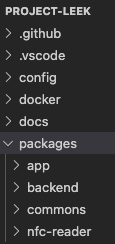
\includegraphics[width=3.8cm]{PackageStruktur.png}
  \caption{Orderstruktur}
  \label{fig:Orderstruktur}
\end{wrapfigure}
Die an das Projekt gesetzten Anforderungen machten die Erstellung mehrerer Applikationen notwendig. Neben einer Benutzeroberfläche, auf der die NFC-Tags
verwaltet werden können, musste die Steuerung des NFC-Readers und ein System zur Speicherung der Daten sowie zum Abspielen der Musik entwickelt werden.
Die dafür benötigten Anwendungen wurden als Microservices konzipiert und umgesetzt. Zur Verringerung des Aufwands der Konfiguration und Wartung wurden die einzelnen Microservices in einem Mono-Repository auf GitHub zusammengefasst.
Jeder Service wurde in einem Unterdner in \textit{packages} angelegt (vgl. Abbildung \ref{fig:Orderstruktur}). Der Ordner \textit{app} enthält die Benutzeroberfläche,
\textit{backed} die Datenbankschnittstelle sowie Logik zur Kommunikation mit dem Musik-Streaming-Anbieter und \textit{nfc-reader} die Applikation zum Steuern und auslesen des am Raspberry Pi angeschlossenen NFC-Readers.
Im Ordner commons befinden sich von allen Services gemeinsam genutzte Ressourcen (wie z. B. Modell-Klassen).
Neben den einzelnen Microservices wurden ebenfalls die Dokumentationsdateien wie Setup-Guide, Benutzerdokumentation und Projektbericht im Mono-Repo im Ordner \textit{docs} abgelegt.
Auch die für den Dienst \textit{Docker} benötigten Dateien fanden in dem gleichnamigen Ordner Platz. Die Konfigurationsdateien für \textit{ESLint} und den \textit{Typescript}-Compiler sind im Ordner \textit{config} zu finden.
Auf die Auflistung aller weiteren Dateien wird in diesem Bericht verzichtet. Eine genaue Aufstellung ist dem \textit{GitHub-Repository}\footnote{\url{https://github.com/project-leek/project-leek}} zu entnehmen.
Durch die Zusammenfassung in ein Mono-Repository waren die einzelnen Services für jeden Entwickler jederzeit einfach erreichbar, ohne die Notwendigkeit das Repository zu wechseln.

\subsection{Technologien}
\label{technologien}

\subsubsection{Programmiersprachen}

\paragraph*{TypeScript} $~$ \\
Da alle Teammitglieder bereits Erfahrungen mit JavaScript gesammelt hatten wurde diese zuerst als Programmiersprache vorgeschlagen.
Aufgrund von nicht vorhandener Typisierung wurde sich dann jedoch auf die von Microsoft entwickelte Sprache TypeScript geeinigt. Diese bietet aufgrund des
Aufbaus auf den ECMAScript-6-Standards eine große syntaktische Ähnlichkeit zu JavaScript. Somit fiel das Erlernen der Sprache den Entwicklern relativ leicht.
Durch die starke Typisierung entstehen außerdem weniger Laufzeitfehler, da die entwickelnde Person bereits zur Compile-Zeit auf Typfehler aufmerksam gemacht wird.\cite{Typescript_Typisierung}
Bei der Kompilierung von TypeScript-Code wird dieser zu gültigem JavaScript Code umgewandelt, wodurch auf eine Vielzahl von bereits existierenden JavaScript-Paketen zugegriffen werden konnte.
Außerdem lässt sich Typescript durch Nutzung der Laufzeitumgebung Node.js auch als Backendsprache verwenden und ersparte dem Team damit die Nutzung von verschiedenen Programmiersprachen.


\subsubsection{Frameworks}
Neben der Programmiersprache Typescript setzte das Team verschiedene Frameworks ein, um bei der Entwicklung auf bereits existierenden Lösungen mit weniger Aufwand zu entwickeln.

\paragraph*{Vue.js} $~$ \\
Zur Gestaltung der Benutzeroberfläche für die \textit{leek-box}, die zum Verwalten der NFC-Tags und Steuern der Ausgabegeräte genutzt wird, einigte sich das Team auf die Nutzung des
clientseitigen JavaScript-Webframeworks \textit{Vue.js}\footnote{\raggedright\url{https://vuejs.org/}}
Dieses wurde aufgrund seiner guten Dokumentation und seiner flachen Lernkurve gewählt, wodurch sich der Einstieg für Teammitglieder mit weniger Erfahrung in der Web-Entwicklung leichter gestaltete.
Außerdem bietet das in Vue.js verwendete Entwurfsmuster MVVM (Model View ViewModel) den Vorteil, dass die designaffineren Entwickler sich eher mit dem Frontend beschäftigen können,
während andere am Logik-Code arbeiten. Im Vergleich zu anderen Webframeworks gilt es, laut Benchmarks außerdem als sehr performant.\cite{Vue_Performance}

\paragraph*{Tailwind CSS} $~$ \\
Zur effizienteren Gestaltung der Benutzeroberfläche entschied sich das Team für das Utility-First-Framework \textit{TailwindCSS}\footnote{\raggedright\url{https://tailwindcss.com}}.
Dieses bietet im Vergleich zu anderen CSS-Frameworks wie \textit{Bootstrap} mehr Flexibilität, da statt vorgefertigten Komponenten vielseitig verwendbare Utility-Klassen zur Verfügung gestellt werden,
über die das Design definiert werden kann. So kann das Aussehen von Elementen innerhalb des HTML-Codes festgelegt werden.
Damit steigt die Übersichtlichkeit des Frontend-Codes, da keine separaten CSS-Dateien und -Klassen angelegt werden müssen.
\cite{Tailwind_Vorteile}


\paragraph*{FeathersJS} $~$ \\
Bei der Erstellung des Backends entschied sich das Team zusätzlich das Framework \textit{FeathersJS}\footnote{\raggedright\url{https://feathersjs.com/}} einzusetzten.
Dies ermöglicht komfortable CRUD-Zugriffe\footnote{CRUD = \textbf{C}reate-\textbf{R}ead-\textbf{U}pdate-\textbf{D}elete}  auf verschiedene Services, welche zum Beispiel Datenbanken oder externe APIs sein können.
Durch eine vielzahl von Adapatern können so zum Beispiel Daten in einer Datenbank ohne eigene Implementierung der Schnittstelle verwaltet werden.
Es muss lediglich ein Service erstellt werden, der das generische Interface Service mit Typeparameter der zu verwaltenden Klasse implementiert. (vgl. Abb. \ref{fig:MyService})
\begin{figure}[h]
  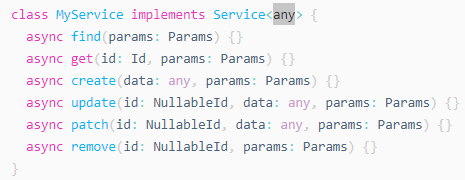
\includegraphics[width=\linewidth]{MyFeathersService}
  \setcaptioncitation{https://docs.feathersjs.com/guides/basics/services.html}
  \caption{Implementierung eines ServicesTest}
  \label{fig:MyService}
\end{figure}
Dabei können verschiedenste Protokolle, wie HTTP oder WebSockets zur Datenübertragung verwendet werden.
Das WebSocket-Protokoll bietet hier den großen Vorteil, dass eine persistente Verbindung zwischen Server und Client (Benutzeroberfläche und Backend) besteht.
So können sowohl Client, wie auch Server jederzeit mit der Datenübertragung beginnen, ohne vorher - wie bei HTTP - jedes Mal eine neue Verbindung aufzubauen zu müssen. \cite{WebSockets}
Dadurch kann der Server alle verbundenen Clients bei einem CRUD-Zugriff informieren, sodass alle ohne erneutes Anfragen der Daten den aktuellsten Zustand übermittelt bekommen.
Wird also beispielsweise ein NFC-Tag von Person A geändert, sieht Person B diese Änderung ohne manuelle Aktualisierung der Seite.
Eine weiteres Feature, welches vom Projektteam genutzt wurde ist die integrierte OAuth-Provider-Abstraktionen, die ein einfaches Authentifizieren mit Diensten, wie beispielsweise \textit{Spotify} bei diesem Projekt ermöglicht.
Dies war z.B. nötig, um die den NFC-Tags zugeordnete Musik abspielen zu können.
Darüber hinaus können so auch Nutzerprofile angelegt werden, ohne persönliche Daten, wie z.B. Namen, Email-Adressen und Passwörter, speichern zu müssen.
Nur Authentifizierungstokens des OAuth-Providers werden in der Datenbank hinterlegt.
So konnte ein besserer Datenschutz für die Nutzenden ermöglicht werden.


\subsubsection{Containervirtualisierung (Docker)}
Es wurde lediglich die Anforderung gestellt, dass die Applikation vor allem für mobile Endgeräte optimiert sein soll.
Auf Basis dieser Anforderung evaluierte das Projektteam bekannte Technologien und recherchierte mögliche Alternativen.
Um die Installation der Box möglichst komfortabel zu gestalten, wird auf die freie Containervirtualisierungssoftware \textit{Docker}\footnote{https://www.docker.com/} gesetzt.
Ohne diese Möglichkeit wäre die Installation aufgrund der drei Microservices (Backend, Reverse-Tunnel und NFC-Reader) sehr aufwändig.
Der Vorteil von Docker besteht darin, dass das Team lediglich eine sogenannte \textit{docker-compose} Datei benötigt, in dem die Konfiguration der Docker-Container beschrieben ist.
Es enthält einen Verweis auf die jeweiligen Container-Images, auf denen die Container aufbauen (z. B. leek-backend). Diese Images enthalten bereits alle notwendigen Abhängigkeiten und Programme,
sodass weitere Installationen seitens der Benutzer:innen nicht erforderlich sind.
Außerdem lässt sich das Verhalten der Images durch Umgebungsvariablen weiter konfigurieren. Durch die einfache Auslieferung bietet Docker außerdem den Vorteil der Reproduzierbarkeit.
So können aufgetretene Fehler problemlos von einem Entwickler nachgestellt werden, da Docker das Betriebssystem des Anwenders von der benötigen Umgebung der leek-box abstrahiert.


\subsubsection{Reverse-Tunnel (ngrok)}
Um verschlüsselt vom Frontend (unter \raggedright\url{https://project-leek.github.io} erreichbar) auf das jeweilige Backend einer \textit{leek-box} zuzugreifen, wird der Reverse-Tunnel Dienst \textit{ngrok}\footnote{\raggedright\url{https://ngrok.com/}} verwendet.
Dies ist notwendig, da moderne Browser eine verschlüsselte Verbindung (mit SSL-Zertifikat) zu allen Komponenten auf der Website verlangen, sobald die Website selbst per SSL geladen wird.
Da das Framwork jedoch nativ kein HTTPS unterstützt, wird \textit{ngrok} verwendet, um die unverschlüsselten Daten durch einen verschlüsselten Tunnel zum Frontend zu schicken. Damit wird die Anforderung der Verschlüsselten Verbindung erfüllt.
Außerdem soll das Backend unabhängig vom lokalen Netzwerk erreichbar sein, ohne dass eine umständliche Portweiterleitung eingerichtet werden muss. Um dies zu leisten, baut das Backend einen Tunnel zu dem Server mit der bekannten Adresse \url{ngrok.io} auf.
Dabei wird eine zufällige Subdomain im Schema \textit{xyz.ngrok.io} angelegt und dem Benutzer in der Konsole des Backends angezeigt. Diese Adresse kann der Benutzer nun im Frontend (\url{https://project-leek.github.io}) eingeben, um sich mit seiner Box zu verbinden.
\colorbox{red}{Hier Schaubild?}

\subsubsection{Externe Bibliotheken}
\paragraph{Spotify Web API} $~$ \\
Um die abspielbaren Songs inklusive Cover-Bildern zu ermitteln und diese abzuspielen ist ein Zugriff auf die API eines Musikstreaming-Dienstes notwendig.
Der vom Kunden vorgeschlagene Anbieter war \textit{Spotify}\footnote{\url{https://www.spotify.com}}.
Um den Zugriff auf die Spotify API zu simplifizieren wurde die Bibliothek \textit{Spotify Web API Node}\footnote{\url{https://github.com/thelinmichael/spotify-web-api-node}} verwendet.
Diese bietet bereits die benötigten Methoden, wie z. B. die zum Suchen eines Songs anhand eines Suchbegriffs.
Neben dem Songtitel und der Spotify-Url werden auch die Künstler und die Adresse des Albumcovers mitgeliefert und konnten von den Entwicklern ohne Mehraufwand genutzt werden.
Auch eine Methode zur Ermittlung der verfügbaren Geräte zum Abspielen der Musik stellt die Bibliothek bereit.

\paragraph{NeDB} $~$ \\
Als Datenbank für dieses Projekt wurde die kostenlos verfügbare JavaScript-Datenbank \textit{NeDB}\footnote{\raggedright\url{https://github.com/louischatriot/nedb}} gewählt.
Sie wird verwendet, um die NFC-Tags, Benutzer und den angeschlossenen NFC-Reader zu verwalten.
\textit{NeDB} ist eine auf \textit{MongoDB}\footnote{\raggedright\url{https://www.mongodb.com/}} aufbauende, sehr schnelle JSON Datenbank.
Sie wurde gewählt, da sie eine geringe Komplexität besitzt und weil \textit{FeathersJS} einen Datenbankadapter für diese Datenbank bereitstellt, was den Zugriff auf die Datenbank sowie die Verwaltung der Daten erleichterte.
Außerdem arbeitet die Datenbank inkrementell, was das Risiko auf sehr große Datenbankdateien minimiert.
Diese Eigenschaft war hilfreich, um die Datenbank auf einem Raspberry Pi betreiben zu können.
Zu Beginn des Projekts diskutierte das Team die Technologien, mit denen die \textit{leek-box} umgesetzt werden sollte.
Der Kunde ließ dem Projektteam hierbei sehr viele Freiheiten.

\subsection{Hilfsmittel}
Im Rahmen des Projekts nutze das Team eine Vielzahl von Hilfsmitteln, die die Zusammenarbeit und Produktivität des Teams steigern sollte.
Diese wurden zum einen zu Beginn des Projektes in einer Gruppendiskussion herausgearbeitet oder als Ergebnis der Retrospektiven erprobt.

\subsubsection{Github \& Github IO}
Da alle Teammitglieder, wie auch die Kunden bereits einen Account bei dem Dienst \textit{GitHub} besaßen, wurde die Entscheidung getroffen, diesen als Hoster für \textit{Git-Remote-Repositories} einzusetzen.
Aufgrund der bereits gewonnenen Erfahrung mit diesem Dienst und der Fokussierung auf quelloffene Software, stellte er für dieses Projekt die ideale Umgebung zur Quellcodeverwaltung und Kollaboration dar.

\paragraph{Kollaboration} $~$ \\
Mit dem Anspruch das Produkt auch nach Projektende fortzuführen, wurden auch die Projektmanagement Funktionen von GitHub verwendet. Die einzelnen Aufgaben bzw. Arbeitspakete (\textit{Issues}\footnote{Da das Team größtensteils den Begriff \textit{Issue} nutzte, wird dieser auch fortlaufend hauptsächlich verwendet.}) wurden in einem \textit{Issue Board} den verschiedenen Arbeitsstatus\footnote{Status = Backlog, Todo, In Progess, Review und Done}
zugeordnet. Außerdem konnten verschiedene Informationen, wie z. B. der Sprint bzw. \textit{Milestone\footnote{Auch hier wird im weiteren Verlauf eher der Begriff Milestone oder Meilenstein verwendet.}} in dem das Ticket abgeschlossen sein soll oder der bearbeitende Entwickler dokumentiert werden.
Da diese Ansicht ebenfalls nach diversen Eigenschaften gefiltert werden kann, konnte sich jeder Entwickler schnell einen Überblick über den aktuellen Projektstand verschaffen.
Das Team setzte zur Unterstützung außerdem den \textit{Renovate-Bot}\footnote{\raggedright\url{https://github.com/renovatebot/renovate}} ein, welcher die Tickets automatisch anhand von verschiedenseten Events verschob und einen Branch anlegt, wenn sich ein Entwickler einem Ticket zuordnet.
\\~\\
Eine weitere Funktionalität von GitHub, die in diesem Projekt genutzt wurden sind die sogenannten \textit{Actions}\footnote{\raggedright\url{https://github.com/features/actions}}.
Sie ermöglichen automatisierte Tests, die den Quellcode und die Anwendung als Gesamtkonstrukt auf verschiedenste Fehler prüfen und frei konfigurierbar sind.
In diesem Projekt wurden die folgenden vier Tests durchgeführt um die Änderungen vor der Übertragung in den Master-Branch zu validieren:
\begin{enumerate}
  \item \textbf{build}: Wird die Software fehlerfrei gebaut?
  \item \textbf{lint}\footnote{Tool zur statischen Codeanalyse}: Ist der Quellcode in gutem Stil geschrieben?
  \item \textbf{test}: Sind die geschrieben Unit-Tests erfolgreich?
  \item \textbf{typecheck}: Sind alle Typen kompatibel?
\end{enumerate}
Sind alle Tests erfolgreich, ist die Änderung technisch nutzbar.
\\~\\
Außerdem wurde die in GitHub existierende Funktionalität der Pull Requests verwendet. Beim \textit{Pushen}\footnote{Hochladen der Änderung vom Entwickler-PC auf das Repositoty auf GitHub}
werden die Änderungen automatisch in dem den Branch betreffenden Pull Request angezeigt (wenn vorhanden).
Jeder Pull Request enthält allgemeine Informationen, welchem Zweck er dient und von wem die Änderung durchgeführt wird. Außerdem wird das Ergebnis der automatisierten Tests (\textit{GitHub Actions}) angezeigt.
Das Projekt ist so konfiguriert, dass die Übernahme der Änderung des Pull Requests nur möglich ist, wenn mindestens zwei andere Entwickler diesen Änderungen
durch Code Reviews zugestimmt haben und alle automatisierten Test erfolgreich abgeschlossen wurden. Ist dies der Fall, kann die Änderung in den Master-Stand übertragen werden.
Für die Code-Reviews wurde ebenfalls die GitHub interne Funktionalität genutzt, die bequeme Änderungsvorschläge ermöglicht.

\paragraph{Github Pages} $~$ \\
Zum Bereitstellen des Frontends der \textit{leek-boxen} wird der Dienst GitHub Pages verwendet. Dieser stellt pro Organisation/Account eine kostenlose Website zur Verfügung.
Die Konigurationsanforderungen für diese Website sind minimal, da der Inhalt der Website an einen Teil des Repositotys gebunden werden kann. In unserem Fall, wird hierfür das \textit{app-package} verwendet.
So bleibt die Website immer aktuell, da sie auf einem eigenen Branch besteht, und der Stand der Website komfortabel durch einen merge vom Master-Branch in den Website-Branch aktualisiert werden kann.
\colorbox{red}{@Anton Please check!}

\subsubsection{Visual Studio Code \& WSL}
Als Entwicklungsumgebung in diesem Projekt wurde \textit{Visual Studio Code} verwendet. VSCode war allen Gruppenmitgliedern bereits bekannt und wurde von vielen auch regelmäßig verwendet.
Die IDE beherrscht den Umgang mit allen für das Projekt benötigten Dateitypen und ist durch eine Vielzahl an kostenlos angebotenen Erweiterungen (Extentions) sehr anpassbar an die Projektbedürfnisse.
So wurden in diesem Fall unter anderem die Erweiterungen \textit{Vetur} (für Vue.js), \textit{LaTeX Workshop}  (für die Erstellung dieses Berichts) und \textit{Tailwind CSS IntelliSense} (Für Auto-Vervollständigung der CSS Klassen von Tailwind) verwendet.
Außerdem bietet \textit{Visual Studio Code} eine komfortable Anbindung\footnote{\raggedright\url{https://code.visualstudio.com/docs/remote/wsl}} an das
\textit{Windows Subsystem für Linux (WSL)}\footnote{\raggedright\url{https://docs.microsoft.com/de-de/windows/wsl/about}}, welches eingesetzt wurde, um eine möglichst homogene Arbeitsumgebung innerhalb des Teams sicherzustellen
und neben der gleichen IDE auch auf Betriebssystemen der gleichen Kernel-Infrastrukur (UNIX) zu arbeiten. Dies erleichterte insbesondere die Arbeit mit \textit{Docker} deutlich.

\subsubsection{Prototyping (Figma)}
Zur Abstimmung auf ein Design für die Benutzeroberfläche wurden vor der Entwicklung Prototypen der benötigeten Komponenten mittels des webbaiserten
Prototyping-Tools \textit{figma}\footnote{https://www.figma.com/} konzipiert. So konnten neben dem Design auch Abläufe in Form von \glqq Click-Dummys\grqq{} erstellt werden und mit dem Kunden abgestimmt werden.
\textit{Figma} wurde verwendet, da es einen kollaborativen Zugriff ermöglicht, kostenlos ist und bereits Erfahrung mit der Plattform bestand

\subsubsection{Lucidchart}
Um Abläufe schon vor dem Prototyping skizziert darstellen zu können wurde außerdem die webbasierte Plattform \textit{Lucidchart}\footnote{\raggedright\url{https://www.lucidchart.com/}} verwendet.
Hier wurde neben der initial erstellten Produktübersicht auch mehrere Aktivitätsdiagramme erstellt, die aus vom Projektteam entwickelten und mit dem Kunden abgestimmten User-Stories entstanden sind.
Diese sind im Anhang unter \colorbox{yellow}{Verweis einfügen!} zu finden.
Auch diese Plattform ermöglicht den gleichzeitigen Zugriff und war den Entwicklern bereits bekannt, was die Notwendigkeit der Einarbeitung eliminierte.
\subsection{Entwicklungszyklus}
Während der Umsetzung der \textit{leek-box} durchlief jedes Teammitglied für jedes \textit{Issue} den am Anfang des Projekts festgelegten und
durch die Retrospektiven optimierten Zyklus.
\\~
Am Anfag steht die Auswahl eines \textit{Issues} aus der Spalte \textit{ToDo} des \textit{Issue Boards}.
Nach Identifikation weist sich der Entwickelnde dem Ticket zu. Daraufhin erstellt der verwendete Bot automatisch einen \textit{Branch}
in dem Schema \textit{[Ticketnummer]-[Ticketname]}. Nun kann mit der Arbeit in \textit{Visual Studio Code} begonnen werden.
\\~
Die Änderungen sollten möglichst kleinschrittig aber sinnvoll \textit{comittet} und anschließend \textit{gepusht} werden.
GitHub erkennt automatisch die neuen \textit{commits} und erfragt, ob ein neuer \textit{Pull-Request} angelegt werden soll.
Dieser hat initial den Status \textit{Open}.
Wenn die Aufgaben des \textit{Issues} noch nicht abgeschlossen sind, wird der Status auf \textit{Draft} gesetzt.
\\~
Nach dem \textit{push} aller Änderungen, wird das Ergebnis der automatisierten Tests (\textit{GitHub Actions}) ermittelt. Treten hierbei Fehler auf,
werden diese geprüft und behoben. Sind alle Tests erfolgreich, betätigt der Entwickelnde die Schaltfläche \textit{Ready for Review}.
Wenn ein:e Entwickler:in, diesen \textit{Pull-Request} sieht, wird ein \textit{Code-Review} durchgeführt.
Hierzu wird der Branch in die IDE geladen und die Funktionalität verifiziert. Anschließend wird die Code-Qualität geprüft.
Dafür werden die geänderten Dateien im Pull-Request betrachtet. Anmerkungen können in Form
von Kommentaren an einzelne oder mehrere Zeilen angefügt werden. Bei Änderungsvorschlägen können diese über eine \textit{suggestion}
getätigt werden. Ist der komplette Code geprüft wird entschieden,
ob die Änderungen angenommen (\textit{approve}) werden oder eine Änderungsanforderung gestellt wird (\textit{Request changes}).
\\~
Im Falle von Änderungsanforderungen werden diese umgesetzt und ein erneutes Review angefordert. Dies geschiet zyklisch, bis die Änderungen angenommen werden.
Sind die Änderungen durch zwei \textit{Code-Reivews} bestätigt worden, werden sie mit der Schaltfläche \textit{Mege into master} übertragen.

\subsection{Testing}
Das Team entschied sich zu Beginn der Produkt-Entwicklung dafür, Tests zur Verbesserung der Codequalität durchzuführen.
Quellcode Tests lassen sich in statische und dynamische Tests unterteilen.

\subsubsection*{Statische Tests}
Im Allgemeinen untersuchen statische Tests nur Textdokumente und betrachten im Gegensatz zu dynamischen Tests nicht das Verhalten zur Laufzeit.
Dies ermöglicht eine häufige und kontinuierliche Nutzung von Tests dieser Art.
Zwei der prominenten Varianten statischer Tests, Linting und Reviews, wurden in diesem Projekt genutzt.

\paragraph*{Linting}$~$ \\
Beim Linting wurde der Code auf syntaktische Korrektheit geprüft.
Auch manche semantische (laufzeitunabhängige) Aspekte wurden untersucht.
So konnten kleinere Denkfehler und Flüchtigkeitsfehler, wie z. B. fehlende Kommata, schnell gefunden und behoben werden.
Hierfür wurde das Analyse-Werkzeug \textit{ESLint}\footnote{\raggedright\url{https://eslint.org/}} genutzt.
Für diese Werkzeug war zusätzlich auch eine Erweiterung\footnote{\raggedright\url{https://marketplace.visualstudio.com/items?itemName=dbaeumer.vscode-eslint}} für die Entwicklungsumgebung verfügbar.
Mit dieser konnten die Ergebnisse des Linting direkt im Code angezeigt werden.
Dies machte den Arbeitsprozess wesentlich zeiteffizienter.
Zusätzlich wurde auch die Erweiterung \textit{Vetur}\footnote{\raggedright\url{https://vuejs.github.io/vetur/}} genutzt.
Diese stellte die selben Funktionalitäten für den Vue-Framework spezifischen Code zur Verfügung.
\\
Darüber hinaus boten diese Erweiterungen auch Formatierungshilfen mit übertragbaren Konfigurationen.
Durch deren Nutzung konnte ein konsistenter Code-Stil innerhalb des Teams ermöglicht werden.
Dies legte den Grundstein für lesbaren Code und ermöglichte successive effizientes Arbeiten.

\paragraph*{Reviews}$~$ \\
Teil des Deployment Cycles waren auch Reviews der aktive Änderungen.
Bei diesen wurde der neue bzw. geänderte Quellcode von mindestens zwei anderen Teammitgliedern überprüft.
Untersucht wurden vor allem semantische Fehler, Lesbarkeit, Wartbarkeit und Vollständigkeit.
Hierfür gab es keinen formalen Plan, allerdings war die Review-Oberfläche von GitHub sehr hilfreich.
In dieser wurde eine Änderungsansicht (\textit{diff}) des zu überprüfenden Codes angezeigt.
So waren alle Teile des neuen Codes auf einen Blick einsehbar.
Darüber hinaus bot die Review-Oberfläche auch die Möglichkeit direkt im Code einzelne oder mehrere Zeilen zu kommentieren.
So konnten auch Änderungsvorschläge gemacht und direkt übernommen werden.
Dies sorgte für einen effizienten Review-Prozess.

\subsubsection*{Dynamische Tests}
Als dynamische Tests wurden in diesem Projekt Anwendungsfall-basierte Tests genutzt.
Bei dieser Art von Test werden auf User-Stories aufbauende Testfälle herangezogen.
Diese Testfälle werden Schritt für Schritt \glqq durchgespielt\grqq.
Dabei wird überprüft, ob das tatsächliche Ergebnis dem erwartetem entspricht.
Die meisten Test  dieser Art wurden als Integrations-Tests durchgeführt.
Bei diesen wurde die Änderungen im Kontext der bestehenden Software getestet.
So konnte vor allem das Zusammenspiel von Frontend und NFC-reader mit dem Backend gut überprüft werden.
Aufgrund der Komplexität dieser Kontrollen wurden diese manuell durchgeführt und nicht automatisiert.
Diese Tests waren Teil des Deployment Cycles und wurden so in den meisten Fällen parallel zu den Reviews durchgeführt.
\\~\\
Ein gewisser Teil der anwendungsfallbasierten Test fand auf der Ebene von Code-Funktionen (\textit{Units}) statt.
Diese Unit-Tests wurden zur einfacheren Wiederholbarkeit automatisiert.
Dazu wurde das JavaScript-Test-Framework \textit{Jest}\footnote{\raggedright\url{https://jestjs.io/}} genutzt.
Dieses wurde gewählt, da sich Tests hiermit sehr intuitiv und ohne großen Lernaufwand schreiben ließen.
Auch diese Tests waren Teil des Deployment Cycles und wurden so bei jedem Pull-Request automatisch ausgeführt.


\subsection{Projekt Meilensteine}

\subsubsection*{Meilenstein 1}
Die Laufzeit des ersten Meilensteins erstreckte sich vom 29.10.2020 bis zum 11.11.2020 und war auf die Planung, Struktur und das Vorgehen des Projektes fokusiert.
%Ziel
Zum Ende des Meilensteins sollte die Struktur und das Grundgerüst für das Projekt fertiggestellt sein.
Hierfür sollte das Konzept der Software-Architektur sowie die genutzten Technologien (später Technologie-Stack genannt) auf Basis einer Anforderungsanalyse mit dem Kunden festgelegt werden.
Außerdem sollten die ersten Tickets in das Backlog eingetragen werden.
Auch musste das Projekt dahingehend geplant werden, dass jedem Teammitglied durchgehend zu bearbeitende Arbeitspakete zur Verfügung standen.
Um ein schnellen und reibungslosen Start für die Entwicklung zu gewährleisten, sollte das Repository entsprechend vorbereitet werden.
%Probleme
Das Team musste das Projekt so entsprechend planen, dass jedes Teammitglied durchgehend sinnvoll arbeiten konnte.
%Lösungen
Durch bereits vorhandene Erfahrung mit verschiedenen Technologie-Stacks und ähnlichen Problemen, wurde sich auf den Technologie-Stack geeinigt
Die verwendeten Technologien sind dem Abschnitt \ref{technologien} zu entnehmen.
Um für jedes Teammitglieds ein sinnvolles kontinuierliches Arbeiten zu gewährleisten, einigte sich das Team auf einen ständig gefüllten Ticket-Pool im Repository, sodass jederzeit selbstständig eine Aufgabe gefunden und bearbeitet werden konnte.
%Product Increment
Das Ergebnis des ersten Meilensteins bestand, abweichend von den späteren, nicht in einem Produkt Inkrement, sondern legte die Grundbausteine für die Entwicklung und das Teamwork.
Neben dem bereits erwähnten Technologie-Stack, wurde als Host für die Applikation ein Raspberry Pi gewählt.
Für die Entwicklung wurde ein Mono-Repository mit \textit{lerna}\footnote{https://lerna.js.org/} aufgesetzt, welches Front- und Backend zusammenfasste.
Durch die Anforderung der Veröffentlichung als Open Source Projekt wurde eine verständliche und hilfreiche Dokumentation nötig, die einem Benutzer die Installation und Verwendung der \textit{leek-box} aufzeigt.
So wurde dem Repository eine einleitende Readme und ein \glqq How to Contribute\grqq{} Guide hinzugefügt.
%Retrospektive
Nach dem ersten Meilenstein fand noch keine nennenswerte Retrospektive statt.

\subsubsection*{Meilenstein 2}
Der zweite Meilenstein wurde für den Zeitraum vom 11.11.2020 bis zum 25.11.2020 angesetzt.
Ziel war es, die ersten Grundbausteine für das Projekt legen.
%Ziel
Damit das Team ein generelles Verständnis des Technologie-Stacks entwickeln konnte, sollte jedes Teammitglied eine \glqq Hello-World\grqq{} Übungsaufgabe absolvieren.
Diese beinhaltete das Anlegen eines Feathers-Services für ein virtuelles Haustier im Backend und die Darstellung im Frontend.
Darüber hinaus sollte sich mit dem Raspberry Pi und dem NFC-Reader auseinandergesetzt werden und die Möglichkeit NFC-Tags auszulesen implementiert werden.
Damit die Entwicklung zeitnah starten konnte, sollten die ersten Mockups für das User Interface erstellt werden sowie die Grundstruktur für den Bericht zu dem Projekt angefertigt werden, damit dieser Projektbegleitend aufgebaut werden konnte.
%Probleme
Zu Beginn ging der im ersten Review geäußerte Kundenwunsch, bereits NFC-Tags auszulesen und anzeigen zu können, unter und stellte so kurzzeitig das rechtzeitige Abschließen der für den Milestone vorgesehenen Tickets in Frage.
Außerdem bereitete die Einarbeitung in die genutzten Technologien einigen Teammitgliedern einige Schwierigkeiten.
%Lösungen
Bereits von Anfang an zeichnete sich durch die hohe Hilfsbereitschaft den anderen Teammitgliedern gegenüber ein hoher Zusammenhalt im Team ab.
Um das vom Kunden gewünschte Feature noch umzusetzen, wurden gegen Ende des Sprints Überstunden geleistet.
%Product Increment
Das Produkt wurde in diesem Meilenstein sinnvoll um ein erstes User Interface erweitert, welches die Tag-ID vom angelegten NFC-Tags anzeigen konnte.
Der NFC-Reader wurde mit dem Raspberri Pi verbunden und als ein auslieferbares Docker Image bereitgestellt.
Auch wurden für die Entwicklung automatisierte Tests erstellt, welche neuen Code auf etablierte Code-Konventionen und Lauffähigkeit überprüften.
%Retrospektive
Vor allem der Einsatz und das Know-How vom Teammitglied Anton wurde hier wertgeschätzt, welcher sich um die Automatisierungen von Tests und Deployment kümmerte.
Auch das Gruppenklima wurde vom Team sehr gelobt, die Zusammenarbeit, Kommunikation und die regelmäßigen Meetings waren liefen sehr gut.
Neu gelernt hat das Team bei diesem Meilenstein vor allem wie Vue, Feathers und Tailwind funktionieren.
Darüber hinaus kamen viele das erste mal Automatisierungsprozessen, Code-Reviews und Pull Request in Kontakt.
Das Team bemängelte bei dem Meilenstein aber auch, dass der Kundenwunsch zu spät behandelt wurde und die Prioritäten falsch gesetzt wurden.
Somit wurde als Verbesserungen für die nächsten Meilensteine eine bessere Koordination und Aufgabenverteilung vorgeschlagen.

\paragraph*{Meilenstein 3}$~$ \\
Vom 25.11.2020 bis zum 17.12.2020 fand die Umsetzung von Meilenstein drei statt.
Die benötigten Anwendungsszenarien und Mockups sollten in diesem Sprint finalisiert werden.
Außerdem sollte der vom Kunden geäußerte Wunsch, dass beim Einlesen eines NFC-Tags die entsprechend hinterlegte Musik abgespielt wird umgesetzt werden.
%Ziel
Dafür musste im Backend ein NFC-Tag mit der jeweiligen Musik angelegt werden.
Um die hohen Anforderungen an die Usability umsetzten zu können, musste sich damit beschäftigt werden, wie Nutzer mit der Anwendung interagieren könnte,.
Daher sollten auch Sequenzdiagramme und weitere Mockups für das User Interface erstellt werden.
Damit jedes Teammitglied auch ohne Hardware arbeiten konnte, sollte es auch möglich sein, das Einlesen von NFC-Tags zu emulieren.
%Probleme
Aufgrund von vorherrschenden Abhängigkeiten mussten Teammitglieder teilweise auf die Vollendung anderer Tickets warten, bevor sie mit diesen begannen.
Ansonsten sind nur kleinere Problematiken, insbesondere bei den Design Mockups, aufgetreten.
Bedingt dadurch, dass das Team nur aus Informatikern bestand, gab es keine ausführlichen Erfahrungen mit Design und Usability Engineering.
%Lösungen
Macio unterstützte das Team, durch die Vermittlung eines Designers ihrer Firma, der die vom Team angefertigten Mockups überarbeitete.
Das Erstellen der Sequenzdiagramme half bei dem Team dabei, das Verhalten eines Nutzers besser einzuschätzen und das User Interface entsprechend zu konzipieren.
%Product Increment
Zusätzlich zu dem Wunsch, beim Anlegen eines NFC-Tags die jeweilig hinterlegte Musik abzuspielen, war auch das Einloggen in einen bestehenden Spotify Account möglich.
Außerdem wurden auf der Startseite die NFC-Tags entsprechend der zugeordneten Gruppe angezeigt.
Jegliche Neuerung auf dem Master wurden nun auch auf Github.io veröffentlicht.
%Retrospektive
Deutlich besser lief in diesem Sprint die Problembewältigung durch Pair Programming, welches die Teamarbeit weiter verbesserte.
Auch der Workflow mit Github, den Pull Request sowie Code Reviews wurde mehr verinnerlicht.
Das Team lernte in diesem Sprint vor allem Vue Hooks kennen, und die Stärken von Feathers in Verbindung mit OAuth.
Festgestellt wurde außerdem, dass einige Tickets weiterhin stark voneinander abhängig waren, weshalb das Bearbeiten einiger Tickets nicht direkt möglich war.
Auf diese Problematik sollte weiterhin geachtete und nach Möglichkeit gegengesteuert werden.
Um das Risiko der Entstehung zukünftiger Probleme zu senken wurde festgelegt mögliche Problemstellungen nicht erst im Standup, sondern so früh wie möglich mitzuteilen.
Genauso sollte neu Gelerntes besser kommuniziert werden, um die Arbeit effizienter zu gestalten.

\subsubsection*{Meilenstein 4} $~$ \\
%Ziel
Zu beginn dieses Meilensteins waren alle Grundlagen gelegt um mit der Umsetzung der Hauptfunktionen zu beginnen.
Es sollten so viele Funktionen des designten User Interfaces umgesetzt werden wie möglich, allerdings lag der Fokus auf einem vollständigem \glqq Add-Tag-Flow\grqq.
Dazu gehörten:
\begin{enumerate}
  \item Scannen des Tags
  \item Vergeben eines eigenen Namens
  \item Auswählen von Musik
  \item Auswählen eines eigenen Bilds
\end{enumerate}
Weiterhin sollten für den nächsten Schritt die Mockups erstellt werden, wie ein Nutzer den Lautsprecher zur Wiedergabe auswählt sowie seine eigene \textit{Leek Box} initial einrichtet.

Um möglichst viel parraleles Arbeiten und Eigentständigkeit der Tickets zu ermöglichen, wurde jede Ansicht in seine einzelnen Komponenten aufgeteilt.
Diese Komponenten sollten für sich alleine stehend funktionieren und so anpassbar sein, dass z.B nur ein Button Komponent entwickelt werden musste, dass auf
allen Ansichten verwendet werden konnte. Es wurde daher erst die grundliegenden Komponenten wie, Buttons, Textfields, Dropdowns entwickelt um aus diesen
Komponenten die Views zu erstellen.

Die Views wurden ebenfalls so in Tickets aufgeteilt, dass möglichst parallel gearbeitet werden konnte.
Beispielsweise wurde die Darstellung auf dem Homescreen, die Auswahl von Infos, Musik und Bild komplett unabhängig voneinander bearbeitet und mit Platzhalterdaten befüllt.
Schließlich wurden alle Komponenten und Seiten zusammengefügt um einen vollständigen Flow zu ermöglichen.
Es konnte nun erfolgreich per UI ein neuer Tag der Datenbank hinzugefügt und in dem HomeScreen angezeigt werden.

\paragraph*{Components}$~$ \\
Für Elemente, die häufig in der Anwendung genutzt werden (Button, Textfield, DropDownList), entwicklete das Team \textit{Vue Components}, die in dem Ordner \textit{uiBlocks} für alle Entwickler leicht zugänglich abgelegt wurden. Diese \textit{components} garantieren, dass die Elemente anpassbar sind und dennoch einem einheitlichen Design folgen. Besonders am Anfag halfen sie dem Entwickler, da sie die Komplexität der Implementierung von Design und Funktionalität senkten. Design und Funktion mussten lediglich einmalig in der \textit{compontent} definiert werden und konnten dann bei Bedarf in den \textit{Views} eingebunden werden. Es musste lediglich der Inhalt über \textit{properties} übergeben werden. Während der fortschreitenden Entwicklung trat allerdings das Problem auf, dass immer mehr Anforderungen an die \textit{components} gestellt wurden und damit immer mehr \textit{Properties} für deren Anpassung notwendig waren. Dies resultierte darin, dass zum Beispiel das \textit{Button-Component} sehr unübersichtlich wurde und redundanten Code enthielt. Aufgrund der verschienden geforderten Größen und Anordungen des Textes und des Bildes, stieg die Anzahl der zu übergebenen Parameter imens, was zu deutlich niedriger Übersichtlichkeit führte. Als Lösung wurde in späteren Meilensteinen eine erneute Analyse durchgeführt die ermittelte, welche Anforderungen ein \textit{component} erfüllen muss. Die Ergebnisse dieser Analyse wurden anschließend genutzt, um den Code zu überarbeiten, wodurch die Übersichtlichkeit der \textit{components} widerhergestellt wurde.

\paragraph*{Umsetzung des Homescreens}
\wrapfiguresafe{r}{0mm}{
  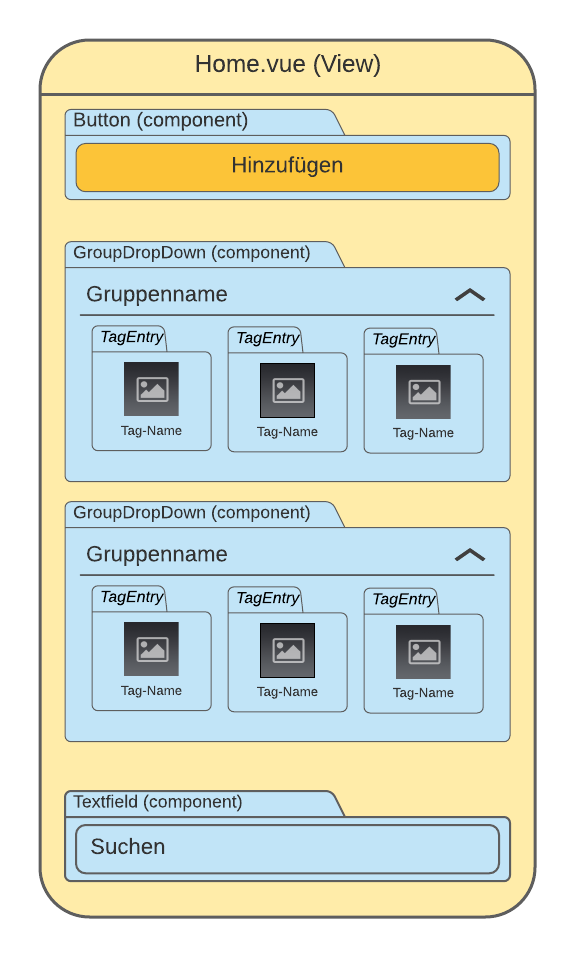
\includegraphics[width=5.9cm]{HomeScreenSchema.png}
}{Schematischer Aufbau Home.vue}
In dem HomeScreen sollten alle angelegten Tags gruppiert angezeigt werden. Hierfür wurden zwei \textit{components} angelegt. Das Erste (\textit{TagEntry.vue})
enthält Bild und Name eines NFC-Tags und konnte in der Anwendung vielseitig widerverwendet werden. Das Zweite \textit{component} mit dem Namen
\textit{GroupDropDown.vue} representiert eine Gruppe, zu der ein NFC-Tag gehört. Pro NFC-Tag in dieser Gruppe wird eine Instanz der
\textit{TagEntry.vue component} in das \textit{GroupDropDown.vue} geladen. Zusätzlich erhielt \textit{GroupDropDown.vue} die Funktionalität es auf- und
zuklappen zu können. Diese \textit{components} werden in \textit{Home.vue} angezeigt. Neben der Einbindung von einer \textit{GroupDropDown.vue} pro Gruppe
wurde im Kopfbereich noch die vom Team erstelle \textit{Button component} verwendet die das Anlegen eines neuen NFC-Tags einleiten soll. Im Fußbereich befindet
sich eine Suchleiste, die das Filtern der angezeigten NFC-Tags ermöglichen Soll. Die beiden letzgenannten Features waren zu diesem Zeitpunkt noch nicht umgesetzt.

\paragraph*{Entwicklung der Tag hinzufügen Funktionalität}
Um dem Benutzer das Hinzufügen von neuen NFC-Tags zur ermöglichen wurde eine neue \textit{View} mit dem Namen \textit{AddTag} erstellt, welche wie auch
der \textit{Home} View in Kopf-, Haupt- und Fußbereich eingeilt ist. Beim Laden der View wird eine neue Instanz der Klasse \textit{NFC-Tag} erstellt.
\\~\\
\wrapfiguresafe{r}{0mm}{
  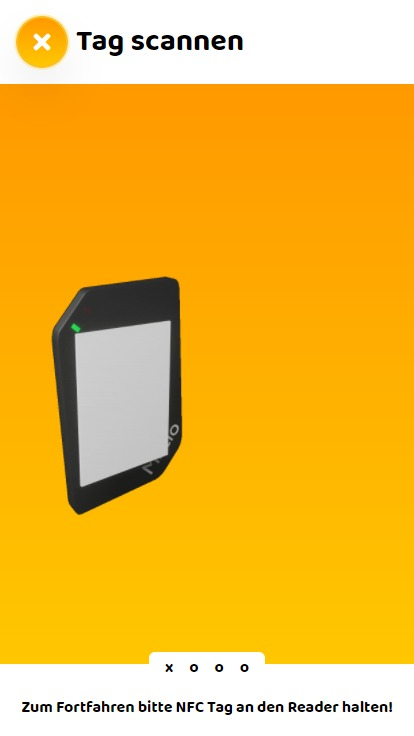
\includegraphics[width=4cm]{AddStepScan.jpeg}
}{AddTag components}
Im Hauptbereich der \textit{View} werden die vier \textit{components} die für die Eingabe der NFC-Tag Daten zuständig sind dynamisch geladen.
Hierfür wird der beim Laden erstellte NFC-Tag (\textit{newTag}) an alle \textit{components} nacheinander weitergegeben und in ihnen mit Informationen gefüllt.
Alle der folgenden \textit{components} beinhalten Validierung für die eingegebenen Daten, sodass sichergestellt wird, dass das \textit{newTag} jederzeit gültige
Daten besitzt. Bei Änderung der Werte in den \textit{components} wird das Event \textit{update:is-valid} ausgelöst und in \textit{AddTag} die
\textit{Disabled}-Eigenschaft des sich in der Fußzeile befindliche Button abhänig vom der Gültigkeit verändert.
\\~\\
\wrapfiguresafe{r}{0mm}{
  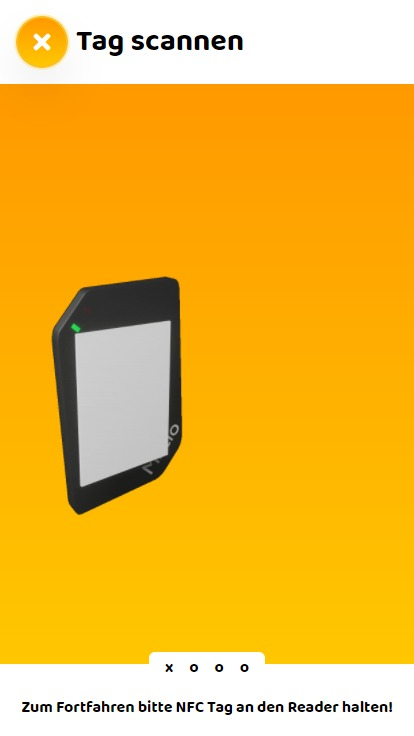
\includegraphics[width=4cm]{AddStepScan.jpeg}
}{Add Step Scan-Tag}
Das Erste \textit{component}, welches in den Hauptbereich geladen wird, ist \textit{TagStepPlaceTagOnReader}. Dieser beinhaltet einen Text und ein \textit{GIF},
welches den Benutzer zum Scannen des NFC-Tags auffordert. Im \textit{TypeScript}-Code wird im \textit{Lifecycle Hook onMounted} an das \textit{patch}-Event des
NFC-Readers der Aufruf der Funktion \textit{attachedTagListener} gebunden. Diese prüft, ob ein NFC-Tag mit dieser ID bereits in der Datenbank vorhanden ist und
leitet den Benutzer in diesem Fall an die \textit{View} zum Bearbeiten des Tags weiter. Ist der NFC-Tag noch nicht angelegt wird die ID an die
\textit{ID-Property} des \textit{newTag} gebunden und das nächste \textit{component} geladen. Beim Entladen von \textit{TagStepPlaceTagOnReader} wird die
Funktion \textit{attachedTagListener} vom \textit{patch}-Event abgemeldet.
\\~\\
Als nächstes wird das \textit{TagStepInfo component} geladen. Es beinhaltet ein \textit{Textbox component} für den Namen des NFC-Readers und ein \textit{DropDown component},
welches die Auswahl der Gruppe ermöglicht. Hierbei kann sowohl aus bereits bestehenden Gruppen gewählt, oder direkt in der \textit{component} eine neue erstellt
werden. Auch diese Informationen werden an die jeweiligen Eigenschaften von \textit{newTag} gebunden und das Event \textit{update:nfc-tag} aufgerufen, wodurch die
\textit{View} den Wechsel zur nächsten \textit{compontent} einleitet.
\\
Hier, in der \textit{TagStepTrack} erhält der Benutzer die Möglichkeit, den Song auszuwählen, der beim Scannen des NFC-Tags abgespielt werden soll. Der gewünschte
Song oder Teile von dessen Titel können in einer \textit{Textbox component} eingeben werden. Daraufhin wird die \textit{Spotify Web Api Node} verwendet, um
zu dem Suchbegriff passende Songtitel mit ihren Albumcovern aus der Spotify-Datenbank anzuzeigen. Aus dem ausgewähltem Song werden die \textit{URL} des
\textit{Tracks} und die \textit{Bild-URL} extrahiert und im \textit{newTag} gespeichert. Anschließend wird durch das Auslösen des \textit{update:nfc-tag}
die letzte \textit{component} in die \textit{AddTagView} geladen.
\\
Zuletzt kann im \textit{TagStepImage} das gewünschte Bild für den NFC-Tag ausgewählt werden. Standardmäßig wird hier das Albumcover des Songs ausgewählt.
Alernativ kann hier auch ein eigenes Bild verwendet werden, welches auf einem Online-Dienst vorliegen muss. Ist dies gewünscht kann in einer entsprechenden
Textbox die \textit{URL} dieses Bildes ausgewählt werden. Zur Bestätigung muss entweder auf das Albumcover oder auf das eigene Bild geklickt werden. Das Erstellen
des Tags kann dann mit einem Klick auf \glqq Anlegen \grqq{} im Fußbereich der \textit{View} abgeschlossen werden.
\\
Der Fußbereich enthält abhänig von der gerade aktiven \textit{component}, \textit{Button components} für \glqq Zurück\grqq{}, \glqq Weiter\grqq{} und
\glqq Anlegen\grqq. Alle diese \textit{components} werden ebenfalls für die Bearbeitung der NFC-Tags widerverwendet.

%Probleme
Durch die angestrebte Unabhängigkeit musste besonders viel Arbeit investiert werden, um die Features miteinander zu verbinden.
Dieser Prozess dauerte länger als erwartet und forderte eine hohes Maß an Kommunikation zwischen den Teammitgliedern.
Teilweise enstanden Wartezeiten und funktionierender Code wurde, über mehrere Merges, unstabil oder defekt.
Kurz vor dem Review noch viel getan werden, um eine reibungslose Präsentation zu garantieren.

%Lösungen
Nachdem die ersten großen Merges abgeschlossen wurde, entschied das Team eine interne und anonyme Evaluation der Teammitglieder zu starten.
Jedes Teammitglied hat somit konstruktive Kritik aber auch Lob und Unterstützung erhalten und konnte an seinen Schwächen arbeiten.
Darüber hinaus wurde auch beschlossen, in den folgenden Sprints die Menge an zu bearbeitenden Issues besser festzulegen.
%Product Increment
Das Produkt wurde um die Grundfunktionen erweitert.
Es ist nun möglich, Tags anzulegen und entsprechend für diese Namen, Musik und ein Bild festzulegen.
Genauso ist es dem Nutzer nun möglich, alle angelegten Tags zu durchsuchen.
Es wurde weiterhin auch das Design Mockup von dem von macio gestellten Designer in Vue größtenteils umgesetzt.
Gleichzeitig wurden hierbei die Komponenten zur einfacheren Verwendung als möglichst allgemeine Vue Komponenten angelegt, um ein einheitliches Design zu ermöglichen.
Für die Entwickler wurden auch die automatisierten Tests um einen Test auf Typsicherheit erweitert.
%Retrospektive
Besonders gut gefiel dem Team das Teamklima, vor allem des ehrliche Miteinander.
Trotz Komplikationen und Probleme konnte dem Kunden am Ende ein funktionierendes Product Increment geliefert werden.
Pull Requests und Tickets wurden besser beschrieben, sodass Probleme verständlicher waren.
Vor allem durch das interne Team Review wurde die Zusammenarbeit weiter verbessert.
Das Team konnte das Wissen zu Vue, vor allem die Themen Reaktivität, Events und Kommunikation zwischen Komponenten ausbauen.
Stark bemängelt wurde der Scope des Meilensteins.
Das Zeitmanagement war an dieser Stelle nicht gut, es wurde sich zu viel vorgenommen und man hatte am Ende zu wenig Zeit.
Das Team stimmte hier überein, dass eine bessere Planung sowie Abstimmung für die nächsten Meilensteine notwendig wäre.
Auch sollte eine frühere interne Deadline gesetzt werden, damit nicht kurz vor dem Sprintende noch viele Fehler auftreten und behoben werden müssen.
Um insgesamt auch die Arbeit kontinuierlicher zu gestalten, sollten Aufgaben in kleinere Probleme aufgeteilt werden.

\subsubsection*{Meilenstein 5} $~$ \\
Der Meilenstein fünf vom 14.01.2021 bis zum 28.01.2021 sollte die Entwicklung am Produkt weitgehend zu abschließen, sodass sich das Team auf den Bericht fokussieren konnte.
%Ziel
Geplant war, die letzten Anwendungszenarien final umzusetzen, sodass die letzten beiden Meilensteine höchstens zum Beheben kleinerer Fehler benötigt werden würden.
Somit war das Ziel die Umsetzung einer Oberfläche für die Einstellungen der \textit{Leek Box} selbst als auch der einzelnen Tags.
Die User Interface Elemente sollten, sofern noch nicht geschehen, ein einheitliches Design erhalten.
Auch sollte die Dokumentation zur Bedienung der \textit{Leek Box} fertiggestellt sein und die Arbeit für den Bericht begonnen werden.
%Probleme
Wie beim vorherigen Meilenstein gestaltete sich auch hier das Zeitmanagement schwierig.
Gegen Ende fehlte es an Zeit, um neu umgesetzte Tickets auf Fehler zu testen und entsprechend fehlerfrei dem Kunden zu präsentieren.
%Lösungen
Als Lösung für dieses Problem beschloss das Team dem Kunden im Review weniger neue Features vorzustellen als geplant.
%Product Increment
Das Produkt Inkrement enthielt die implementierten Einstellungen der \textit{Leek Box}, die es dem Nutzer ermöglichen, den Wiedergabelautsprecher auswählen, die jeweilige Leek Box zu verwalten und sich von Spoitfy abzumelden.
Auch wurde ein Setup Guide angefertigt, sodass ein Nutzer selbstständig eine eigene \textit{Leek Box} einrichten könnte.
Bei dem Design wurden alle Unstimmigkeiten beseitigt.
%Retrospektive
Insgesamt hat das Team sich an dieser Stelle vor allem über das sehr positive Feedback des Kunden gefreut.
Auch wurde die Produktivität des Teams sehr gelobt.
Das Team konnte außerdem weitere Vue Funktionen kennenlernen.
Problematisch war es, dass manche Tickets von mehreren gleichzeitig oder nacheinander bearbeitet wurden, sodass Arbeit teilweise doppelt erledigt wurde.
Außerdem erfolgte die Kommunikation von größeren Änderung an jedes Teammitglied teilweise nur lückenhaft.
Lösungsvorschläge waren Verbesserung des Zeitmanagements durch \colorbox{yellow}{???} und eine bessere Kommunikation durch Festhalten von größeren Änderungen in den Pull Requests und Markierung aller Gruppenmitglieder.

\subsubsection*{Meilenstein 6} $~$ \\
Mit dem Meilenstein sechs vom 28.01.2021 bis zum 15.02.2021 sollte die Entwicklung beendet und der Fokus komplett auf den Bericht gelegt werden, sodass der nächste und letzte Meilenstein für die letzten Korrekturen im Bericht genutzt werden konnte.
%Ziel
Neben der Fokussierung auf den Bericht sollte auch das User Interface auf einheitliches Design überprüft und die Entwicklung und Fehlerbehebung abgeschlossen werden.
%Probleme
\colorbox{red}{TODO:}schlauchiger start in den report

%Lösungen
\colorbox{red}{TODO:}Welche Lösungen haben wir gefunden?

%Product Increment
Als letzte Änderungen am Produkt hat nun der Nutzer die Möglichkeit, verschiedene Leek Boxen auszuwählen bzw. neu eingerichtete Leek Boxen mit seinem Konto zu verbinden.
Die letzten Bugfixes wurden umgesetzt sowie wurden die letzten Details aus dem Design Mockup übernommen.
%Retrospektive
\colorbox{red}{TODO:}Was haben wir dabei gelernt? Neue Erkentnisse? Neue Sichtweisen?
Was lief gut, neu gelernt, was lief nicht so gut, was verbessern?

\subsubsection*{Meilenstein 7} $~$ \\
Der finale Meilenstein sieben vom 15.02.2021 bis zum 05.03.2021 sollte nur noch die letzten Korrekturen des Berichtes und Vorbereitung der Finalen Abgabe beinhalten.
\colorbox{red}{TODO:}Kurze Einleitung, von, bis
%Ziel
\colorbox{red}{TODO:}was haben wir uns vorgenommen, was war das ziel, was wollten wir schaffen?
%Probleme
\colorbox{red}{TODO:}welche prrobleme sind aufgetreten?

%Lösungen
\colorbox{red}{TODO:}Welche Lösungen haben wir gefunden?

%Product Increment
\colorbox{red}{TODO:}Was ist am Ende dabei rumgekommen?

%Retrospektive
\colorbox{red}{TODO:}Was haben wir dabei gelernt? Neue Erkentnisse? Neue Sichtweisen?
Was lief gut, neu gelernt, was lief nicht so gut, was verbessern?


\section{Fazit}
\subsection{Probleme, Lösungen, Erkenntnisse}
\colorbox{red}{TODO: Finde TITEL:} Fazit oder nur Erkenntnisse oder oder?
\colorbox{red}{Besseres Intro zum Kapitel?}
Das Projekt Informatik gab einen realistischen Einblick in die Arbeitswelt.
Das Team musste sich klassischen Alltagsproblemen stellen, Lösungswege finden und konnte wichtige Erkenntnisse für die Zukunft daraus ziehen.
Auch Coding-Entwurfsmuster und -Konventionen wurden neu erlernt und praktisch angewandt.
$~$ \\
%Einarbeitung in neue Technologien
Zu Beginn des Projektes bestand eine größere Differenz, inwieweit die einzelnen Teammitglieder mit den jeweiligen Technologien vertraut waren.
Insbesondere die Projektstruktur bereitete eine größere Einstiegshürde für viele Entwickler.
Sie wurde durch das automatische generieren von Dateien und Ordnern immer komplexer.
Mit zunehmender Entwicklungszeit und durch die Arbeit an den Teilkomponenten des Mono-Repositorys gewannen die Entwickler jedoch schnell mehr Überblick über die Struktur.
Das Team lernte wie Frameworks und Libraries  z. B. Vue, Tailwind und Feathers sinnvoll und hilfreich eingesetzt werden können.
$~$ \\
%Versionskontrolle und Deployment Cycle
Zwar wurde den Studierenden im Studium der Vorteil von Versionskontrollsystemen wie Git vermittelt, doch fand sich selten ein praktisches Anwendungszenario, dass Git über die Hauptfunktion der Versionierung hinaus sinnvoll genutzt hat.
Dieses Projekt bot erstmals eine sinnvolle Anwendung von \textit{git}.
Die Umsetzungen der gängigen Industriestandarts we z.B Pull-Requests und Code Reviews lehrte uns die Vorteile von Git in einer komplexen Umgebung.
Diese Methoden führten zu folgenden maßgebliche Verbesserungen:
Mit zwei erfordelichen Code Reviews pro Pull Request, konnten Fehler im Code häufiger entdeckt werden und so eine höhere Codequalität erreicht.
Als positiver Nebeneffekt konnten die Reviewer außerdem während des Prozesses neue Funktionen und Codemuster erlernen, zu denen sie bei Bedarf (per Kommentar) Fragen stellen konnten.
Die Gewöhnung an diesen Deployment Cycle brauchte eine gewisse Zeit, fand aber von Sprint zu Sprint immer mehr Wertschätzung im Team.
$~$ \\
%Automatisierte Tests und Deployment
Jeder Pull Request durchlief mehrere automatisierte Tests - sogenannte \textit{Actions} - die den geänderten Code auf Korrektheit in Syntax und simplen Semantischen fragen getestet haben.
Inhaltliche Funktionen der Applikation wurden durch die Tests nicht abgedeckt.
Diese prüften den Quellcode anhand fest eingestellter Testparameter.
Durch diese Tests wurde dem Team viel manuelle Arbeit abgenommen und die Fehlerquelle Mensch minimiert.
Änderungen im Master werden automatisch verarbeitet. Die neue Version des Codes wird auf Github.io veröffentlicht und geänderte Latex Dateien als PDF im eigenen Branch erstellt.
Für Pull Requests wurde ebenfalls eine Vorschau erstellt und auf einer \colorbox{yellow}{temporären} Webseite veröffentlicht.
Dank dieser Automatisierungen konnte sich das Team mehr auf das Weiterentwickeln des Projektes konzentrieren.

%Regelmäßige Standups und Retrospektiven
Durch die regelmäßigen Standups entstand ein Ort für den Austausch von Problemen und Informationen über Fortschritt und neue Funktionen.
So wurde verhindert, dass Probleme untergingen, neues Wissen wurde schneller verbreitet und die gesamte Teamproduktivität verbessert.
Das bei den Retrospektiven entstandene Feedback erwies sich als sehr wichtig für das Teamklima.
Auch die hierbei angesprochenen Probleme und Verbesserungsvorschläge wurden vom Team als sehr wertvoll für die nächsten Sprints erkannt und entsprechend adaptiert.

%Kommunikation und Eigeninitiative
Anfänglich hat sich das Team zu sehr auf die Standups, als alleiniges Kommunikationsmittel verlassen, wodurch die Absprache zwischen den Teammitgliedern nur selten statt gefunden hat.
Der Umfang erster Tickets war deutlich zu groß.
Die Komplexität eines Tickets hat Teammitglieder davon abgehalten sich mit der Thematik zu beschäftigen.
Da konkrete Fragen bei einem gänzlich neuen Thema schwierig zu formulieren sind, wurde oft komplett auf Hilfe verzichtet und das Ticket zur Seite gelegt.
Lösungsansätze wurden gemeinsam in den Retrospektiven erarbeitet.
Weiterhin konnte offen über Probleme gesprochen werden, indem teaminterne Evaluationen stattgefunden haben.

%Planung, Zielsetzung und Einschätzung
Größere Probleme hatte das Team mit dem Zeitmanagment der einzelnen Ticket.
Während eines Milestones wurden manchmal nicht alle geplanten Tickets fertiggestellt, oder es wurde nachträglich zu viel in den Sprint neu Aufgenommen.
Beides resultierte in Überstunden und zu wenig Zeit fürs Testen am Ende eines Meilensteins.
Aus diesen Erfahrungen, hat das Team gelernt wie wichtig es ist die Planung des Meilensteins und dessen Tickets besonders sorgfältig zu gestalten.
So hat das Team sich auch vorgenommen, mindestens zwei Tage vor einem Sprintende alle für den Sprint benötigten Tickets fertiggestellt zu haben.
Dadurch sollte genügend Zeit geschaffen werden, um Tickets auf Korrektheit zu testen und konfliktfrei in den Master Branch mergen zu können.
Auch wenn die Lösung dieses Problem hätte effizienter behandelt werden können, war diese Methode angesichts der knappen Projektlaufzeit die effektivste.
\subsection{Ausblick}
\newpage
\section{Anhang}
\colorbox{red}{BEISPIEL, DELETE THIS} Buchreferenz \cite{Literaturbeispiel:tom} oder Seitenref \cite{google}
\printbibliography
\end{document}
